% TODO eval all datasets for ldof ped mc, ldof pd sc
%TODO: explain statistical method: precission, recall, f1, density
%TODO: statistics: performance of selected set of methods applied on all datasets: HS_PD_SC, LDOF_PD_SC (classic), LDOF_PED_MC, LDOF_SD, LDOF_SED, SRSF_PED, SRSF_SED
%TODO: statistics: influence of lambda using LDOF_PD
%TODO: statistics: LDOF_PED_SC vs LDOF_PD_SC
%TODO: statistics: LDOF_PED_SC vs LDOF_PED_SC
%TODO: statistics: LDOF_PD_MC vs LDOF_SD
%TODO: statistics: LDOF_PED_MC vs LDOF_SED
%TODO: statistics: best case - tweak paras for a dataset.

%TODO: varying anzahl cluster: chair bonn/cerealbox 2:12, 3d lodf, unmerged results (ped sc, mc, mache plot anz.cluster/f1 score je methode plus prec-recall plot je methode
%TODO: mache overall performance stat. wenn standard params

\chapter{Results}
Finally, in this last section we describe how we evaluate our generated segmentations. Principally, the quality of a resulting segmentation is measured by comparing it against a manually drawn ground truth segmentation image. \\ \\
In the following the term $\textbf{P-affinity}$ refers to an affinity matrix generated by a product distance combination method. That means, that the affinity was produced by either $\textbf{PD}$ or $\textbf{PED}$. Please refer to the section $\ref{sec:affinity_matrix_impl}$ on page $\pageref{sec:affinity_matrix_impl}$ to re-read the definition of these modes. 

\section{Default Parameter Assignments}
\label{sec:spectral_clustering_parameters}
Even though our pipeline mainly consists of tree main components, that is the flow computation stage, the affinity matrix generation stage and the segmentation stage, it exhibits a large amount of parameters that have to be specified. This issues makes it tedious to use our implementation, especially, when running the pipeline repeatedly over and over again (e.g. during our experiments). Therefore, we aim at reducing the number of free parameters in our pipeline by providing certain default assignments. \\ \\
In this section we address this problem of default parameter assignments. In particular we explain which parameter gets what default value assigned to and why. \\ \\
Our motion segmentation pipeline exhibits many parameters since it consists of several stages such as the flow generation- affinity matrix computation- segmentation stage. Moreover, every stage implements different techniques to approach its specified tasks. Hence, a user has to specify both, which pipeline combination should be run and what parameter values of an specific method should be used. To get the overall picture of this complexity we illustrate all available \textit{pipeline combinations} in figure $\ref{fig:pipeline_combinations}$. 
\begin{figure}[H]
\begin{center}
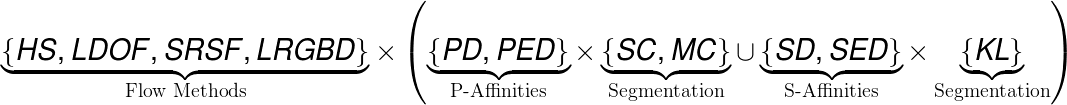
\includegraphics[width=1\linewidth] {evaluation/pipeline_combinations}
\end{center}
\caption[Pipeline Combinations]{A listing of all available pipeline combinations. Our pipeline implements a series of flow methods (4), various affinity computation modes (4) and different segmentation techniques (3). In total, there are $4 \times (2 \times 2 + 2 \times 1) = 24$ different combinations available. However, not every component mode can be combined with any other. For example \textit{S-affinities} can only be used in combination with the \textit{Kernighan-Lin Heuristic} (KL). }
\label{fig:pipeline_combinations}
\end{figure}
In the following we give a brief description of several default assignments used in different pipeline stages. \\ \\
For generating the flow fields we rely on existing implementations as described in section $\ref{sec:generate_of}$. We do not attempt to modify any parameter settings while utilizing those flow methods and thus strictly rely on their default settings. A summary about these flow methods can be found in section $\ref{sec:impl_optical_flow}$ on page $\pageref{sec:impl_optical_flow}$. \\ \\
Before tracking trajectories as described in section $\ref{sec:trajectory_tracking}$, we initially have to extract their feature locations (Sec. $\ref{sec:tracking_candidates}$). The resulting feature extraction is determined by a parameter defining the sparsity of the sampling rate, indicating to use only every $k-th$ feature. Throughout performing our experiments we will be using $k$ equals to 8. This choice is justified by the fact that using a smaller sampling rate would not enhance the result's quality and negatively influence the overall runtime, whereas larger values would cause the opposite. \\ \\
Next some words about choosing defaults for the affinity matrix generation stage. Before computing a $\textit{P-affinity}$, either by running the mode \textit{PD} or $\textit{PED}$, we have to specify a certain value $\lambda$. This parameter is used in equation $\ref{eq:prod_dist_affinity}$ and acts as a scale of the similarity between two trajectories. In the follows we use$\footnote{We determined the defaults by trying out different values for $\lambda$ and took those which yielded the visually most promising results. Please note that this kind of parameter selection is by no means optimal.}$ $\lambda$ equals $0.01$ when running $PD$ and $\lambda = 50$ when running the affinity mode $PED$. The reason for using different $\lambda$ values is because PED and PD have different scales. As we can see $\lambda$ takes different powers to ten. However the exact choice of this scale does not matter$\footnote{Meaning, that it \textit{does not matter} regarding using a different mantissa, since it will not affect the final outcome of the affinity matrix drastically.}$ that much as long as it close to the same power to ten value as its corresponding default. \\ \\
When having a closer look at the computed affinities, we observe, that approximately one third of the trajectory neighbors have similarity large enough to have a big influence on it. Therefore, we decided to set the number of closest neighbors per trajectory equals one third of the total neighbors. An example is shown of such affinities is shown in figure $\ref{fig:cars_w}$. A dark pixel indicates a low affinity between two trajectories and bright regions indicate large affinities. \\ \\
In order to generate S-affinities we rely on the definition of equation $\ref{eq:sum_dist}$, which is used to compute distances between trajectories. However, this equation is parameterized by several weights $\beta$. In this work we use the exactly the same $\beta$ values as defined in the paper $\cite{KB15b}$, which are equal to
\begin{equation}
\begin{aligned}
\bar{\beta}_0 = 6 \text{, } \beta_0 = 2 \text{, } \beta_1 = \beta_3 = -0.02 \text{ and } \beta_2 = -4
\end{aligned}
\end{equation}
In our experiments we set the dummy vertex count in the Kernighan-Lin partitioning method always equals zero. \\ \\
For every segmentation methods, we specified the \textit{cluster count} they are supposed to solve for equals to two times the number of an estimated number of moving objects present in the target dataset. In other words the cluster count $CC$ is an personal estimate and defined as
\begin{equation}
	\text{CC} = 2 \times \text{Estimated Moving Objects in Dataset}
\label{eq:cc_def} 
\end{equation}
This estimation approach only takes into account very clearly, distinct moving objects and is thus probably underestimating the real moving object count. \\ \\
Segmentation methods that rely on P-affinities are utilizing a certain number of eigenvectors resulting from the eigenvalue decomposition of the Laplacian. For this eigenvector Count (EV) we use twice the number of the clusters the methods are supposed to solve for, i.e. this count is defined as
\begin{equation}
	\text{EV} = 2 \times \text{CC}
\end{equation}
Moreover, when using the MC segmentation, we set the default of its data- and smoothness relaxation parameter $\nu$ used by its energy term (defined in equation $\ref{eq:min_cut_energy_revisited}$) equals to the dimension of the affinity matrix times $10^{-6}$. Again, this value has been determined by simply trying out various assignments. Furthermore, we observed that it is sufficient to run about 10-20 iterations until MC converges. Therefore, we conservatively assign the number of iterations $\text{MC}_i$ equals 20. \\ \\
Unless stated otherwise we rely on those parameter default parameter specifications to generate out results. Moreover, in section $\ref{sec:parameter_experiments}$, we offer a statistical justification for the default choices of $\lambda$, $\text{CC}$, $\text{EV}$ and $\text{MC}_i$.

\section{Datasets}
\label{sec:datasets}
In this section we introduce the dataset we were using for generating our results. Our dataset are a diverse collection of videos, originating from various source. Some videos were captures by Microsoft's Kinect, some by Asus' Xtion. Some were manually captures and again others are from other authors. In particular the cars dataset is from the Middlebury dataset$\footnote{See \url{http://vision.middlebury.edu/stereo/data/}}$ and datasets prefixed by \textit{Bonn} are from Bonn's RGB-D Rigid Multi-Body Dataset $\footnote{See \url{http://www.ais.uni-bonn.de/download/rigidmultibody/}}$. \\ \\
We aim to work with a diverse collection of datasets. Meaning that we want to use datasets that capture different types of motions, are recorded in-and outdoor scenes and are captured by a static or moving cameras. Also, our implementation should be able to generated segmentations for long as well as for short sequences. \\ \\
Regularly, a dataset consists of the frames of a RGB-D video and the corresponding depth-and color camera calibrations. Moreover, for a selected set of frames we manually have drawn$\footnote{To draw these ground truth images using Gimp.}$ ground truth (\textbf{GT}) images. Please notice that all GT images were drawn according to the painter's opinion and thus do probably not truly correspond to the real ground truth motion. Each color in such a GT image belongs to a moving object. However, the color \textit{black} has a spacial meaning and marks pixels that are not certain to which moving object they belong to. Such pixel locations are ignored during our evaluation. \\ \\
In the following a listing of our datasets, listing three of its frames, one of its ground truth motion segmentation images, a list of properties and a brief description what is happening in the video:
\begin{itemize}
\item \textbf{Cars}: \textbf{frames}: 19, \textbf{resolution}: $480 \times 640$, \textbf{depths}: No 
\begin{figure}[H]
\begin{center}
\subfigure[Frame 1]{
   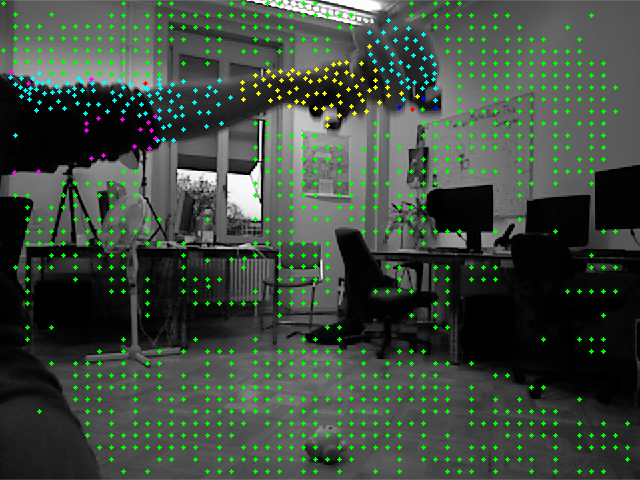
\includegraphics[width=0.22\linewidth] {evaluation/datasets/cars/1}
}
\subfigure[Frame 10]{
   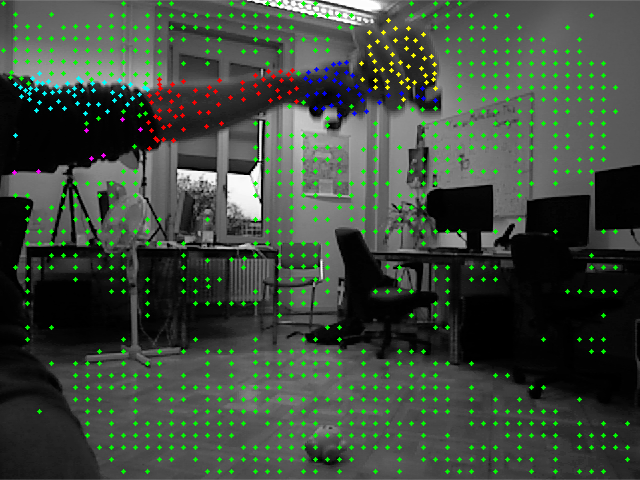
\includegraphics[width=0.22\linewidth] {evaluation/datasets/cars/10}
}
\subfigure[Frame 19]{
   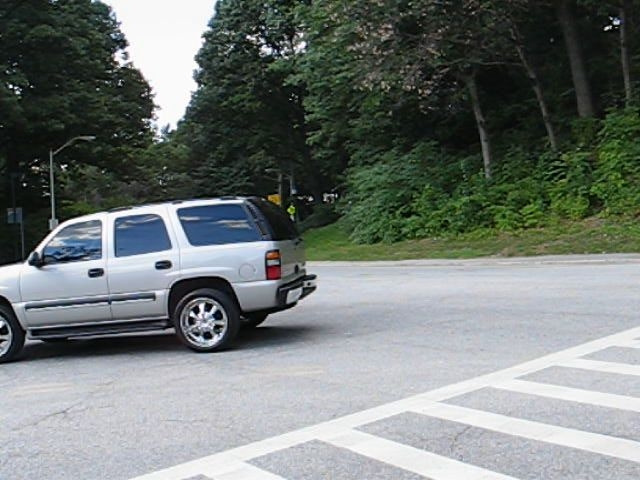
\includegraphics[width=0.22\linewidth] {evaluation/datasets/cars/19}
}
\subfigure[GT Frame 1]{
   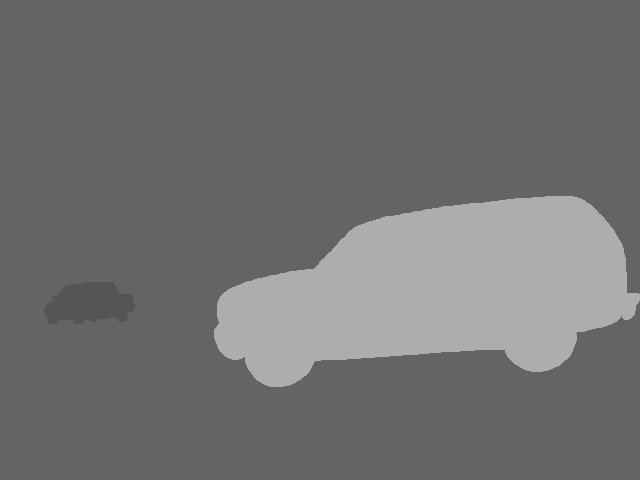
\includegraphics[width=0.22\linewidth] {evaluation/datasets/cars/gt1}
}
\end{center}
\caption[Dataset Bonn Cars]{An outdoor scene showing two cars, both moving to the left. One in the front and the other in the background. The camera is static.}
\label{fig:eval_datasets_cars}
\end{figure}
\item \textbf{Bonn Watercan}: \textbf{frames}: 58, \textbf{resolution}: $480 \times 640$, \textbf{depths}: Yes
\begin{figure}[H]
\begin{center}
\subfigure[Frame 4]{
   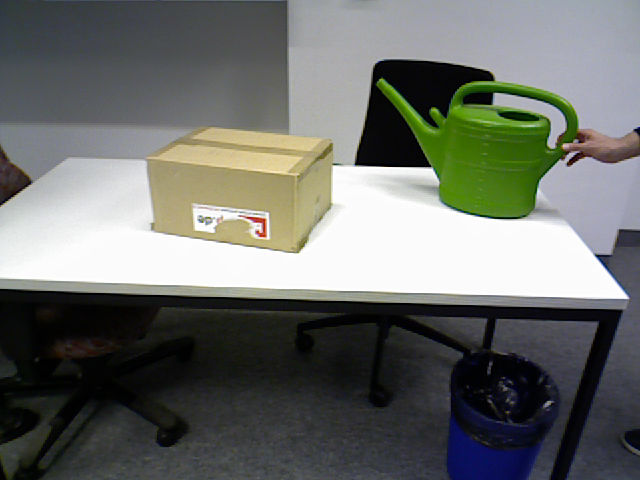
\includegraphics[width=0.22\linewidth] {evaluation/datasets/bonn_watercan/4}
}
\subfigure[Frame 31]{
   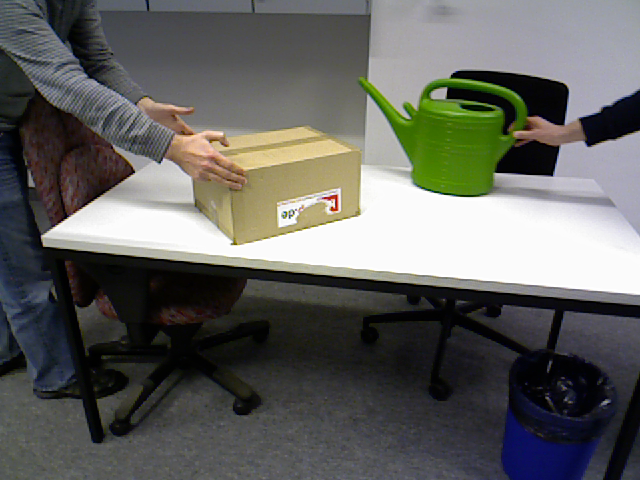
\includegraphics[width=0.22\linewidth] {evaluation/datasets/bonn_watercan/31}
}
\subfigure[Frame 58]{
   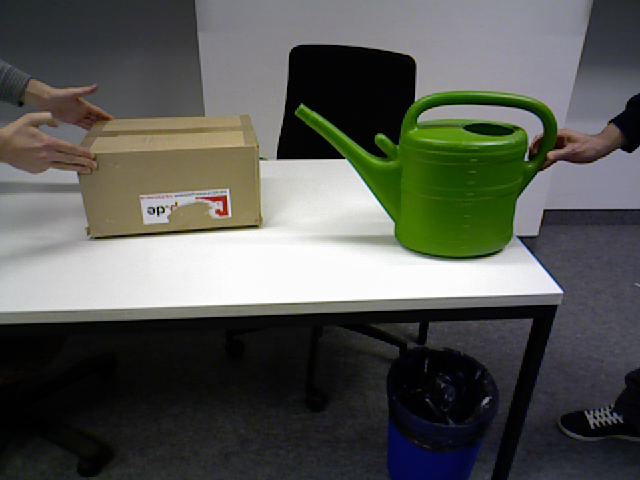
\includegraphics[width=0.22\linewidth] {evaluation/datasets/bonn_watercan/58}
}
\subfigure[GT Frame 4]{
   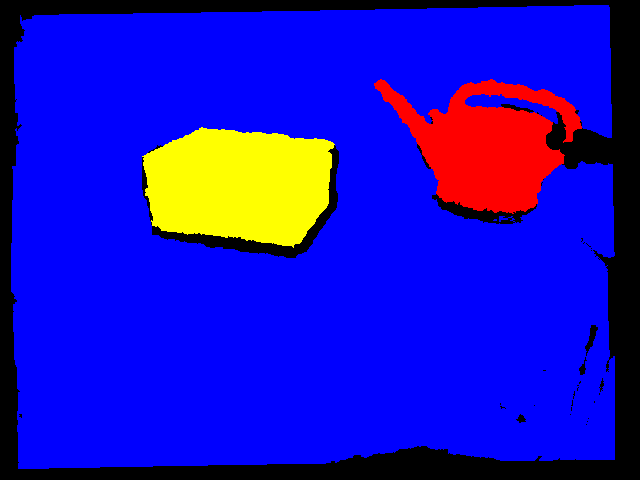
\includegraphics[width=0.22\linewidth] {evaluation/datasets/bonn_watercan/gt4}
}
\end{center}
\caption[Dataset Bonn Watercan]{An indoor scene showing two men psuhing different objects on a table. First, the man on the right side moves a water can along the table, then after a while the second man moves a packet from the left side of the table to its center. The camera is slightly shaking.}
\label{fig:eval_datasets_bonn_watercan}
\end{figure}
\item \textbf{Bonn Chairs}: \textbf{frames}: 58, \textbf{resolution}: $480 \times 640$, \textbf{depths}: Yes
\begin{figure}[H]
\begin{center}
\subfigure[Frame 15]{
   \includegraphics[width=0.22\linewidth] {evaluation/datasets/bonn_chairs/15}
}
\subfigure[Frame 30]{
   \includegraphics[width=0.22\linewidth] {evaluation/datasets/bonn_chairs/30}
}
\subfigure[Frame 45]{
   \includegraphics[width=0.22\linewidth] {evaluation/datasets/bonn_chairs/45}
}
\subfigure[GT Frame 15]{
   \includegraphics[width=0.22\linewidth] {evaluation/datasets/bonn_chairs/gt15}
}
\end{center}
\caption[Dataset Bonn Chairs]{An indoor scene showing a man moving a chair. First, he moved it to the left, then he rotates it slightly. The camera is slightly shaking.}
\label{fig:eval_datasets_bonn_chairs}
\end{figure}
\item \textbf{Bonn Cerealbox}: \textbf{frames}: 101, \textbf{resolution}: $480 \times 640$, \textbf{depths}: Yes
\begin{figure}[H]
\begin{center}
\subfigure[Frame 40]{
   \includegraphics[width=0.22\linewidth] {evaluation/datasets/bonn_cerealbox/40}
}
\subfigure[Frame 60]{
   \includegraphics[width=0.22\linewidth] {evaluation/datasets/bonn_cerealbox/60}
}
\subfigure[Frame 80]{
   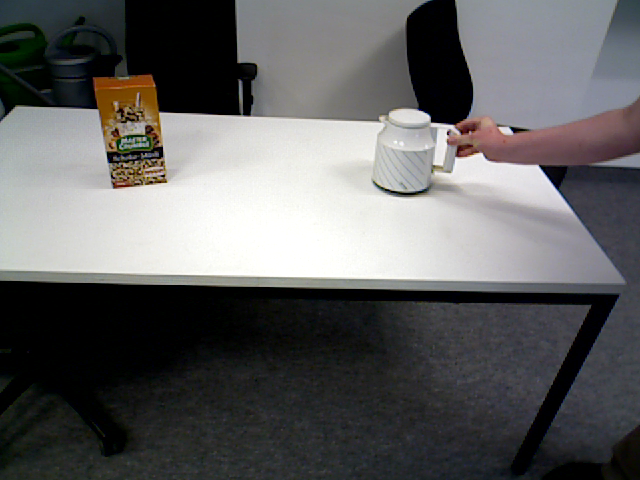
\includegraphics[width=0.22\linewidth] {evaluation/datasets/bonn_cerealbox/80}
}
\subfigure[GT Frame 40]{
   \includegraphics[width=0.22\linewidth] {evaluation/datasets/bonn_cerealbox/gt40}
}
\end{center}
\caption[Dataset Bonn Cerealbox]{An indoor scene showing a man moving a cup on table. The camera is slightly moving.}
\label{fig:eval_datasets_bonn_cerealbox}
\end{figure}
\item \textbf{Statue}: \textbf{frames}: 111, \textbf{resolution}: $480 \times 640$, \textbf{depths}: Yes
\begin{figure}[H]
\begin{center}
\subfigure[Frame 30]{
   \includegraphics[width=0.22\linewidth] {evaluation/datasets/statue/30}
}
\subfigure[Frame 60]{
   \includegraphics[width=0.22\linewidth] {evaluation/datasets/statue/60}
}
\subfigure[Frame 90]{
   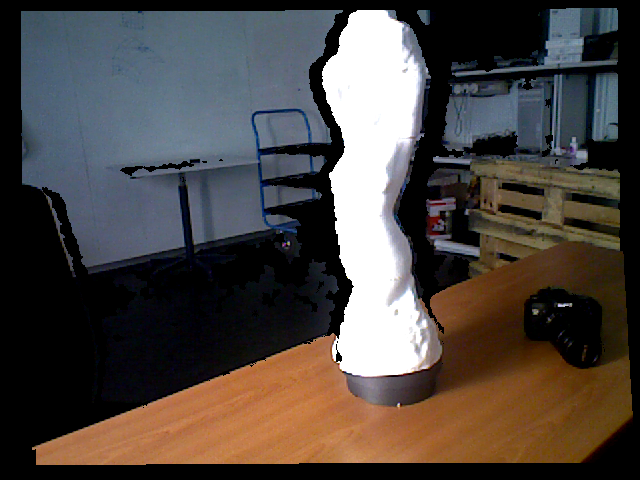
\includegraphics[width=0.22\linewidth] {evaluation/datasets/statue/90}
}
\subfigure[GT Frame 30]{
   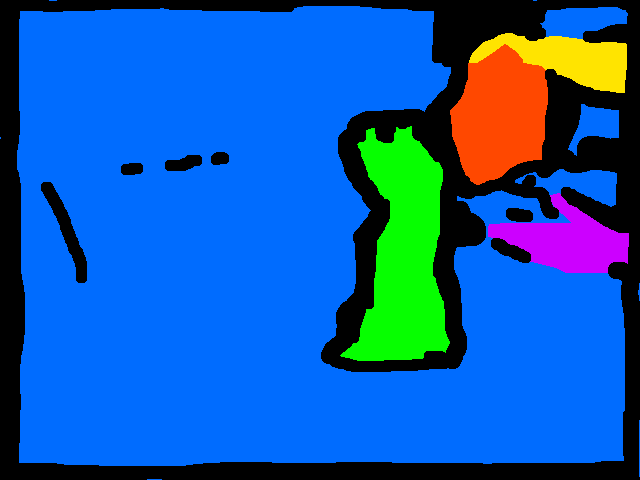
\includegraphics[width=0.22\linewidth] {evaluation/datasets/statue/gt30}
}
\end{center}
\caption[Dataset Statue]{An indoor scene a rotating statue. After a whole a man removes the upper part. We only see the man's hand. The camera is static.}
\label{fig:eval_datasets_statue}
\end{figure}
\item \textbf{Waving Arm}: \textbf{frames}: 104, \textbf{resolution}: $480 \times 640$, \textbf{depths}: Yes
\begin{figure}[H]
\begin{center}
\subfigure[Frame 20]{
   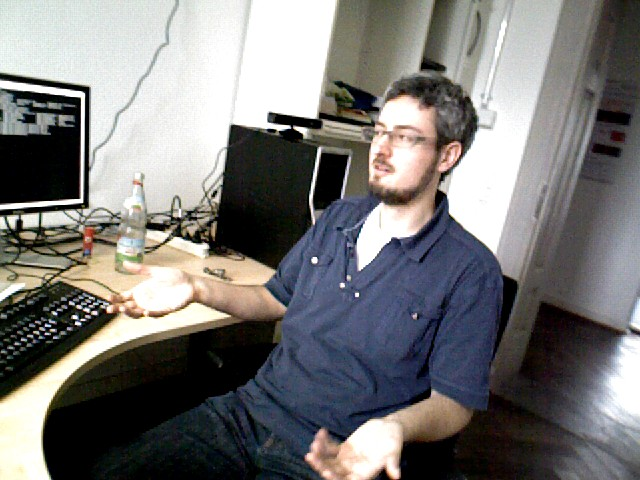
\includegraphics[width=0.22\linewidth] {evaluation/datasets/wh/20}
}
\subfigure[Frame 30]{
   \includegraphics[width=0.22\linewidth] {evaluation/datasets/wh/30}
}
\subfigure[Frame 40]{
   \includegraphics[width=0.22\linewidth] {evaluation/datasets/wh/40}
}
\subfigure[GT Frame 40]{
   \includegraphics[width=0.22\linewidth] {evaluation/datasets/wh/gt40}
}
\end{center}
\caption[Dataset Waving Hand]{An indoor scene showing a waving arm. The camera is static.}
\label{fig:eval_datasets_waving_hand}
\end{figure}
\item \textbf{Two Chairs}: \textbf{frames}: 61, \textbf{resolution}: $512 \times 424$, \textbf{depths}: Yes
\begin{figure}[H]
\begin{center}
\subfigure[Frame 15]{
   \includegraphics[width=0.22\linewidth] {evaluation/datasets/two_chairs/15}
}
\subfigure[Frame 40]{
   \includegraphics[width=0.22\linewidth] {evaluation/datasets/two_chairs/40}
}
\subfigure[Frame 60]{
   \includegraphics[width=0.22\linewidth] {evaluation/datasets/two_chairs/60}
}
\subfigure[GT Frame 15]{
   \includegraphics[width=0.22\linewidth] {evaluation/datasets/two_chairs/gt15}
}
\end{center}
\caption[Dataset Two Chairs]{An indoor scene showing two spinning chairs. The camera is static.}
\label{fig:eval_datasets_two_chairs}
\end{figure}
\item \textbf{One Chair}: \textbf{frames}: 101, \textbf{resolution}: $512 \times 424$, \textbf{depths}: Yes
\begin{figure}[H]
\begin{center}
\subfigure[Frame 45]{
   \includegraphics[width=0.22\linewidth] {evaluation/datasets/one_chair/45}
}
\subfigure[Frame 60]{
   \includegraphics[width=0.22\linewidth] {evaluation/datasets/one_chair/60}
}
\subfigure[Frame 75]{
   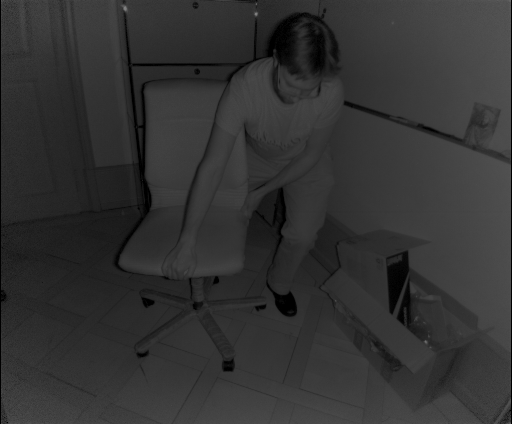
\includegraphics[width=0.22\linewidth] {evaluation/datasets/one_chair/75}
}
\subfigure[GT Frame 45]{
   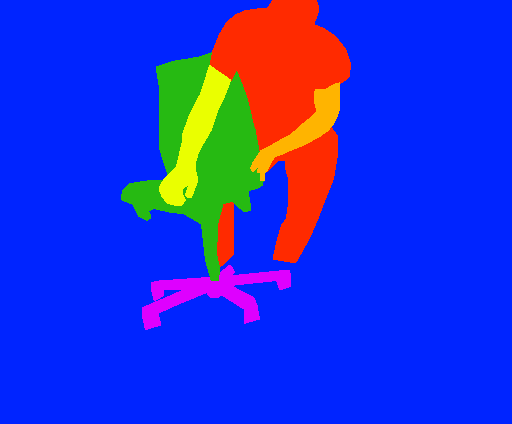
\includegraphics[width=0.22\linewidth] {evaluation/datasets/one_chair/gt45}
}
\end{center}
\caption[Dataset One Chair]{An indoor scene a man lifting a chair and spinning its lower part. The camera is static.}
\label{fig:eval_datasets_one_chair}
\end{figure}
\end{itemize}

\section{Segment Merger}
\label{sec:seg_merger}  
In this section we describe our technique to reduce oversegmentations produced by our pipeline. Our goal is to offer a mechanism that allows to evaluate the maximal potential of pipeline. However, some segmentation results are not clearly defined, such as fast movements resulting from non-rigidly moving objects. An good example of this problem case is when we attempt to segment a video showing a waving hand. That is rationale why we want to merge unclear segments. Moreover, we only allow to merger sparse segmentations, since our dense segmentation approach is basically blurring the sparse segments and thus is not yielding comparable results$\footnote{The more post-processing steps are added the more obfuscated the final segmentation quality gets.}$. This stage is invoked before running the evaluation program, implemented as a post-processing stage. \\ \\
Usually, the results generated by our pipeline exhibit an oversegmentation when comparing them against their ground truth. An example of such an oversegmentation is illustrated in figure $\ref{fig:merger_result_b}$. Ideally, before evaluating the quality, we would like to refine our over-segmented results in a way such that the total number of unnecessary or unclear segments is reduced. Therefore we want to merge  merge segments causing an oversegmentation. We achieve this by comparing the generated segments against a manually drawn ground truth image. For any generated segment we determine their best matching ground truth segment with respect to their overlapping parts. A conceptual visualization of our merging technique is visualized in figure $\ref{fig:merger_result}$. Please note that such a merging technique is just a hack. A more sophisticated method is described for merging clusters is presented in $\cite{OB14b}$.
\begin{figure}[H]
\begin{center}
\subfigure[Ground Truth Segmentation]{
   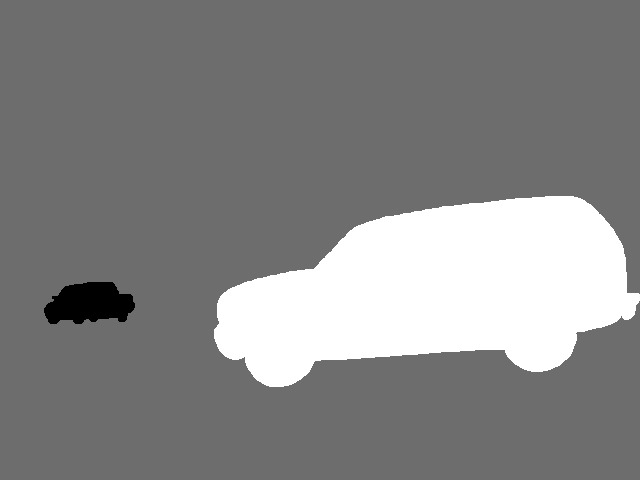
\includegraphics[width=0.47\linewidth] {implementation/merger/mask}
   \label{fig:merger_result_a}
}
\subfigure[Generated Segmentation]{
   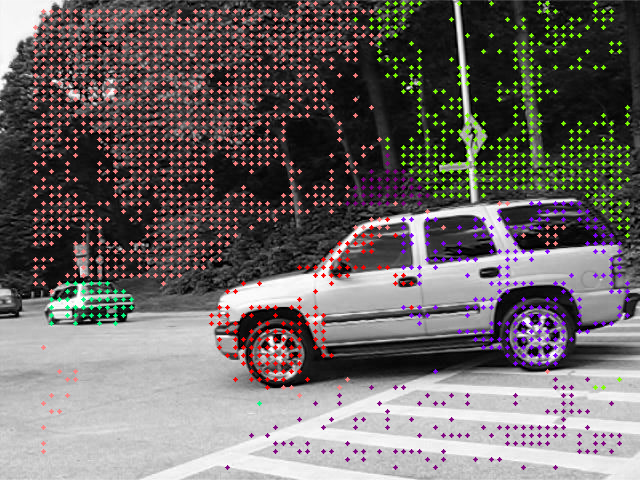
\includegraphics[width=0.47\linewidth] {implementation/merger/oversegmentation}
   \label{fig:merger_result_b}
}
~
\subfigure[Overlay Ground Truth / Segmentation]{
   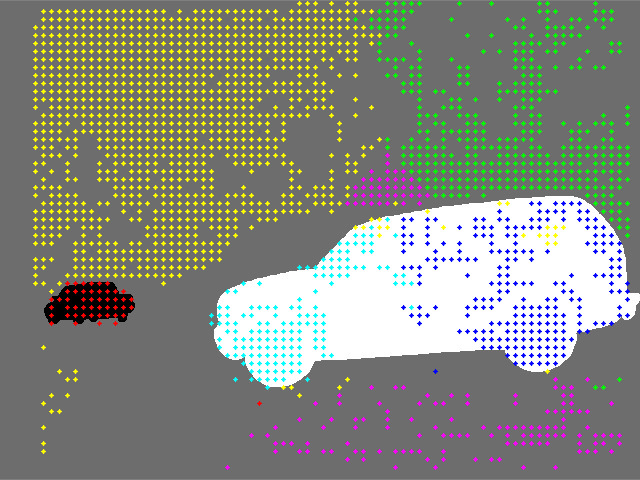
\includegraphics[width=0.47\linewidth] {implementation/merger/mask_segments_overlay}
   \label{fig:merger_result_c}
}
\subfigure[Merged Segmentation]{
   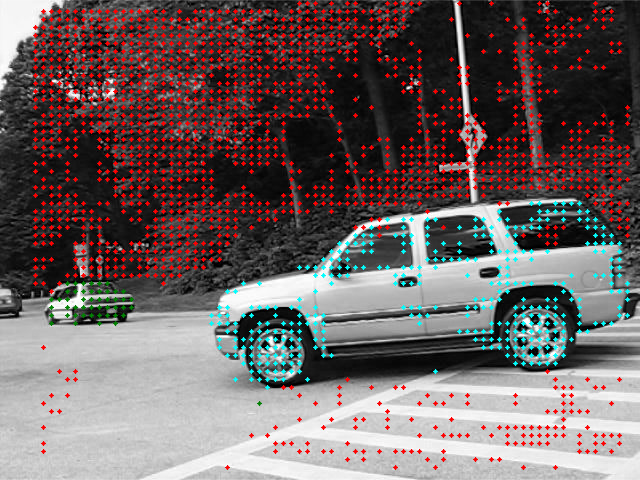
\includegraphics[width=0.47\linewidth] {implementation/merger/merged}
   \label{fig:merger_result_d}
}
\end{center}
\caption[Segmentation Merger]{Visualization of our segment merger's input and output. As an input it expects a ground truth segmentation (see figure $\ref{fig:merger_result_a}$) and a generated oversegmentation (see figure $\ref{fig:merger_result_b}$). As output it yields the merged segmentation as shown in subfigure $\ref{fig:merger_result_c}$.}
\label{fig:merger_result}
\end{figure}
A segmentation $S$ is basically a set of points in which every point is assigned to a certain segment identifier. In the following let us denote $S_j$ as the subset of points in $S$ that belong to the segmentation label $j$. Similarly, let $M$ denote the set of all ground truth points with their corresponding mask labels and $M_i$ the set of all points that belong to the ground truth mask $i$. To compute the merged segments we do the following: For every segment $S_j$ in $S$ we determine its best matching ground truth segment $M_i$ as defined in equation $\ref{eq:merging_label_formula}$. 
\begin{equation}
i = \argmaxl_{M_i \in M} \left\vert{S_j \cap M_i}\right\vert
\label{eq:merging_label_formula}
\end{equation}
The idea is to find the ground truth mask $i$ that yields the most point intersections with the currently considered segment $S_j$. Next, we update every point in $S_j$ by setting their segment label to $i$. After doing so we have computed the merged segmentation version of the initial oversegmentation. An example is shown in figure $\ref{fig:merger_result_c}$.

\section{Methodology}
\label{sec:methodology}
In this section we give a brief description about the methodology used to perform our experiments. \\ \\
We want to quantitatively evaluate the quality of segmentations produces by running different pipeline combinations. In particular we propose to evaluate the quality of how well moving objects were segmented. We use the datasets described in section $\ref{sec:datasets}$. Produced motion segmentations are compared against available ground truth images. While running the pipeline we rely on the defaults described in section $\ref{sec:spectral_clustering_parameters}$.\\ \\
Before evaluating the performance of generated segmentations, we run our segment merger, which is described in section $\ref{sec:seg_merger}$, as a post-processing step. The merged segments are quantitatively evaluated using different statistical measures. After running the merger, each GT object is assigned to at most one label. Therefore, the evaluation measures can be computed independently per object. In particular, for each segmentation result we compute their precession, recall and their f1 score by comparing them against their ground truth. The definition of these measures is listed in equation $\ref{eq:statistical_measures}$. 
\begin{equation}
\begin{aligned}
	& \text{precision} = \frac{\text{TP}}{\text{TP} + \text{FP}} \\
	& \text{recall} = \frac{\text{TP}}{\text{TP} + \text{FN}} \\
	& F_1 \text{ Score} = 2 \left( \frac{\text{precision} \times \text{recall}}{\text{precision} +\text{recall}} \right)
\end{aligned}
\label{eq:statistical_measures}
\end{equation}
The final reported outputs is the average value of these measured over all foreground objects. \\ \\
Finally some words about how we determined the quantities $TP$, $FP$ and $FN$. We only have to iterate over all points in every cluster and compare them against an available ground image. While doing so we count their true positives (\textbf{TP}), false negatives (\textbf{FP}) and their false negatives (\textbf{FN}). The exact definition of these quantities is listed in equation $\ref{eq:statistical_counts}$. For a given label $\alpha$ these measures are defined as:
\begin{equation}
\begin{aligned}
	\textbf{TP} &:= \text{Samples correctly labeled $\alpha$} \\
	\textbf{FP} &:= \text{Samples incorrectly labeled $\alpha$} \\
	\textbf{FN} &:= \text{Samples that were labeled $\alpha$ in GT but are attributed to a wrong label.}
\end{aligned}
\label{eq:statistical_counts}
\end{equation}
A detailed explanation of these measures can be found in the background section $\ref{sec:on_statistics_bg}$ on page $\pageref{sec:on_statistics_bg}$. \\ \\
One last note: During our evaluations we want to determine the quality of segmentations and the influence of design choices regardless of additional post-processing steps. Since our dense motion segmentation method basically performs a blurring on the sparse segmentation, and thus the quality is arbitrary influenced, we disallow using dense segmentations in our quantitative evaluation.

\section{Experiments}
In this section we list the results of a series of experiments we performed running our pipeline on the presented dataset from section $\ref{sec:datasets}$ on page $\pageref{sec:datasets}$. The results are evaluated according the previously explained measures from section $\ref{sec:methodology}$ on page $\pageref{sec:methodology}$. \\ \\
For performing our experiments we used MacBook Pro. The hardware specifications of this machine are listed in table $\ref{tab:used_hardware_specs}$. 
\begin{table}[H]
\centering
\begin{tabular}{|l|c|}
\hline
\multicolumn{2}{|c|}{\textbf{Hardware Specifications}} \\ \hline
\textbf{CPU} & 2.5 GHz Intel Core i7 \\ \hline
\textbf{Threads} & 8 \\ \hline
\textbf{MEMORY} & 16 GB 1600 MHz DDR3 \\ \hline
\textbf{GPU} & Intel Iris Pro 1536 MB \\ \hline
\end{tabular}
\caption{A listing of the hardware specifications of the used machine to produce the results.}
\label{tab:used_hardware_specs}
\end{table}
The first series of experiments examines the influence of certain pipeline parameters. In particular we legitimize the choice for our default parameter assignments. Next, we have study the behaviour and quality of segmentations when altering our flow estimation methods. The main experiment is the evaluation of some strong pipeline combinations applied on all of our datasets. Finally, we try to find the best pipeline combinations for each stage.

\subsection{Parameter Experiments}
\label{sec:parameter_experiments}
In this section we describe a series of experiments that address our default parameter selection choice. In particular it acts as a justification of our choices and should demonstrate their legitimization.

\subsubsection{Examine Influence of Cluster Merger}
For the following experiment we examine the influence of our cluster merger. In particular we visually evaluate the influence of this merging step. In this experiment we only use LDOF flows. The visual results are shown in figure $\ref{fig:eval_raw_vs_merged}$.
\begin{figure}[H]
\begin{center}
\subfigure[Raw PD SC]{
   \includegraphics[width=0.2\linewidth] {evaluation/bonn_chairs_c_10_segmentations_f_30/ldof_pd_sc}
}
\subfigure[Merged PD SC]{
   \includegraphics[width=0.2\linewidth] {evaluation/bonn_chairs_c_10/ldof_pd_sc}
}
\subfigure[Raw PD MC]{
   \includegraphics[width=0.2\linewidth] {evaluation/bonn_chairs_c_10_segmentations_f_30/ldof_pd_mc}
}
\subfigure[Merged PD MC]{
   \includegraphics[width=0.2\linewidth] {evaluation/bonn_chairs_c_10/ldof_pd_mc}
}
~
\subfigure[Raw PED SC]{
   \includegraphics[width=0.2\linewidth] {evaluation/bonn_chairs_c_10_segmentations_f_30/ldof_ped_sc}
   \label{fig:eval_bonn_chairs_raw_segmentations_frame_30_c}
}
\subfigure[Merged PED SC]{
   \includegraphics[width=0.2\linewidth] {evaluation/bonn_chairs_c_10/ldof_ped_sc}
   \label{fig:bonn_chairs_c_10_d}
}
\subfigure[Raw PED MC]{
   \includegraphics[width=0.2\linewidth] {evaluation/bonn_chairs_c_10_segmentations_f_30/ldof_ped_mc}
   \label{fig:eval_bonn_chairs_raw_segmentations_frame_30_d}
}
\subfigure[Merged PED MC]{
   \includegraphics[width=0.2\linewidth] {evaluation/bonn_chairs_c_10/ldof_ped_mc}
   \label{fig:bonn_chairs_c_10_e}
}
~
\subfigure[Raw SD KL]{
   \includegraphics[width=0.2\linewidth] {evaluation/bonn_chairs_c_10_segmentations_f_30/ldof_sd_kl}
   \label{fig:eval_bonn_chairs_raw_segmentations_frame_30_e}
}
\subfigure[Merged SD KL]{
   \includegraphics[width=0.2\linewidth] {evaluation/bonn_chairs_c_10/ldof_sd_kl}
   \label{fig:bonn_chairs_c_10_d}
}
\subfigure[Raw SED KL]{
   \includegraphics[width=0.2\linewidth] {evaluation/bonn_chairs_c_10_segmentations_f_30/ldof_sed_kl}
   \label{fig:eval_bonn_chairs_raw_segmentations_frame_30_f}
}
\subfigure[Merged SED KL]{
   \includegraphics[width=0.2\linewidth] {evaluation/bonn_chairs_c_10/ldof_sed_kl}
   \label{fig:bonn_chairs_c_10_e}
}
\end{center}
\caption[Bonn Chairs Segmentations Frame 30]{Raw-and merged segmentations produced by our pipeline when running all modes on the Bonn Chairs dataset using LDOF flows.}
\label{fig:eval_raw_vs_merged}
\end{figure}

The statistical measurements are listed in table $\ref{tab:eval_stat_raw_merged}$



\subsubsection{Examine Varying Cluster Count}

\begin{figure}[H]
\begin{center}
\subfigure[2 Clusters]{
   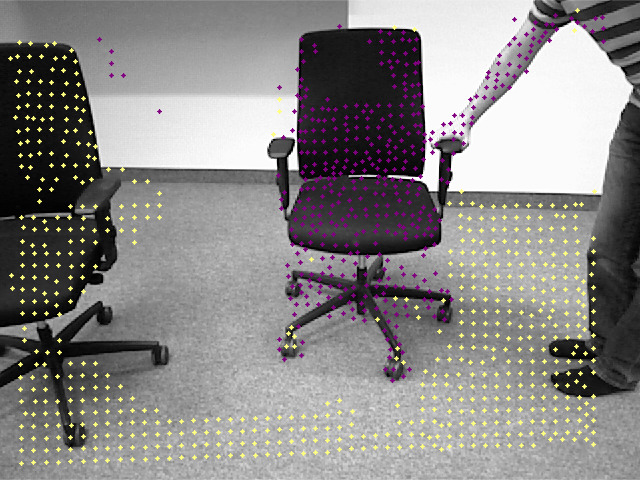
\includegraphics[width=0.31\linewidth] {evaluation/bonn_chairs_ldof_varying_c_sed/f_30_c_2}
   \label{fig:bonn_chairs_sed_varyingclusters_a}
}
\subfigure[3 Clusters]{
   \includegraphics[width=0.31\linewidth] {evaluation/bonn_chairs_ldof_varying_c_sed/f_30_c_3}
   \label{fig:bonn_chairs_sed_varyingclusters_b}
}
\subfigure[4 Clusters]{
   \includegraphics[width=0.31\linewidth] {evaluation/bonn_chairs_ldof_varying_c_sed/f_30_c_4}
   \label{fig:bonn_chairs_sed_varyingclusters_c}
}
~
\subfigure[5 Clusters]{
   \includegraphics[width=0.31\linewidth] {evaluation/bonn_chairs_ldof_varying_c_sed/f_30_c_5}
   \label{fig:bonn_chairs_sed_varyingclusters_a}
}
\subfigure[6 Clusters]{
   \includegraphics[width=0.31\linewidth] {evaluation/bonn_chairs_ldof_varying_c_sed/f_30_c_6}
   \label{fig:bonn_chairs_sed_varyingclusters_b}
}
\subfigure[7 Clusters]{
   \includegraphics[width=0.31\linewidth] {evaluation/bonn_chairs_ldof_varying_c_sed/f_30_c_7}
   \label{fig:bonn_chairs_sed_varyingclusters_c}
}
~
\subfigure[8 Clusters]{
   \includegraphics[width=0.31\linewidth] {evaluation/bonn_chairs_ldof_varying_c_sed/f_30_c_8}
   \label{fig:bonn_chairs_sed_varyingclusters_a}
}
\subfigure[9 Clusters]{
   \includegraphics[width=0.31\linewidth] {evaluation/bonn_chairs_ldof_varying_c_sed/f_30_c_9}
   \label{fig:bonn_chairs_sed_varyingclusters_b}
}
\subfigure[10 Clusters]{
   \includegraphics[width=0.31\linewidth] {evaluation/bonn_chairs_ldof_varying_c_sed/f_30_c_10}
   \label{fig:bonn_chairs_sed_varyingclusters_c}
}
\end{center}
\caption[Bonn Chairs SED Segmentations for Varying Cluster Count]{A visualization of the real segmentations when running \textit{SED KL} on the \textit{bonn chairs} dataset.}
\label{fig:bonn_chairs_sed_varyingclusters}
\end{figure}

\begin{figure}[H]
\begin{center}
\subfigure[Recall / Precision Plot]{
   \includegraphics[width=0.47\linewidth] {evaluation/bonn_chairs/avg/avg_rec_prec}
   \label{fig:bonn_chairs_plot_avg_stat_a}
}
\subfigure[Cluster Count / F1 Score Plot]{
   \includegraphics[width=0.47\linewidth] {evaluation/bonn_chairs/avg/avg_clusters_f1}
   \label{fig:bonn_chairs_plot_avg_stat_b}
}
\end{center}
\caption[Chair 3 Cast avg statistic plots]{Plots of the average performance of the four methods PED SC, PD MC, PED SC and PED MC for a varying number of clusters. The left plots shows the recall/precision plot and the figure on the right shows the F1 score alongside the number of clusters.}
\label{fig:bonn_chairs_plot_avg_stat}
\end{figure}

\subsubsection{Examine Convergence of MC}
In the graph of figure $\ref{fig:two_chairs_ped_mc_iterations}$ we see a plot of the convergence rate of the MC segmentation method. The more iterations we run, the higher the F1-Score gets. However, we also observe, that the F1 Score is converging already after 3 iterations. This matches with our assumption that no more than 5 to 10 iterations have to be run when using the MC segmentation method.
\begin{figure}[H]
\begin{center}
\includegraphics[width=0.47\linewidth] {evaluation/two_chairs/performance_iter/iter_f1}
\label{fig:two_chairs_ped_mc_iterations_b}
\end{center}
\caption[Convergence Rate MinCut Segmentation]{Visualizing the convergence rate of MC. We observe, that the more iterations are run, the higher the F1-Score gets. However}
\label{fig:two_chairs_ped_mc_iterations}
\end{figure}
\begin{figure}[H]
\begin{center}
\subfigure[1 Iteration]{
   \includegraphics[width=0.22\linewidth] {evaluation/two_chairs/iters/iter_1}
}
\subfigure[2 Iterations]{
   \includegraphics[width=0.22\linewidth] {evaluation/two_chairs/iters/iter_2}
}
\subfigure[3 Iterations]{
   \includegraphics[width=0.22\linewidth] {evaluation/two_chairs/iters/iter_3}
}
\subfigure[5 Iterations]{
   \includegraphics[width=0.22\linewidth] {evaluation/two_chairs/iters/iter_5}
}
\end{center}
\caption[Convergence Segmentations Two Chairs]{Visualizing the convergence of the MC segmentation method.}
\label{fig:two:chairs_segmentations_ped_mc_iters}
\end{figure}

\subsubsection{Examine $\lambda$ Default}
In this experiment we examine the influence of the parameter $\lambda$, which is used to scale P-affinities. In particular, we legitimize its described standard parameter choices. For different values of $\lambda$ we generate P-affinity matrices for both of its run-modes, PD and PED. In this experiment, the trajectories tracking uses LDOF flows, since other authors (e.g. in $\cite{OB14b}$) have reported its effectiveness. Our results are listed in table $\ref{tab:varying_lambda_experiment}$.
\begin{table}[H]
\centering
\setlength\tabcolsep{4pt}
\begin{minipage}{0.48\textwidth}
\centering
\begin{tabular}{|c|c|c|c|}
\hline
\multicolumn{4}{|c|}{Varying $\lambda$ on PD} \\ \hline
$\lambda$ & \textbf{Precision} & \textbf{Recall} & \textbf{F1 Score} \\ \hline
5 & 11.68 & 10.73\% & 11.18\%  \\ \hline
1 & 15.68 & 11.51\% & 13.28\%  \\ \hline
0.1 & 34.05 & 30.08\% & 31.94\%  \\ \hline
\textbf{0.01} & \textbf{46.37} & \textbf{52.94}\% & \textbf{49.44}\%  \\ \hline
0.001 & 43.00 & 45.67\% & 44.29\%  \\ \hline
0.0001 & 25.11 & 25.78\% & 25.44\%  \\ \hline
\end{tabular}
\end{minipage}%
\hfill
\begin{minipage}{0.48\textwidth}
\centering
\begin{tabular}{|c|c|c|c|}
\hline
\multicolumn{4}{|c|}{Varying $\lambda$ on PED}                        \\ \hline
$\lambda$ & \textbf{Precision} & \textbf{Recall} & \textbf{F1 Score} \\ \hline
100 & 36.60\% & 35.11\% & 35.84\%  \\ \hline
\textbf{50} & \textbf{52.44}\% & \textbf{59.28}\% & \textbf{55.65}\%  \\ \hline
10 & 45.33\% & 52.22\% & 48.53\%  \\ \hline
5 & 53.50\% & 51.02\% & 52.23\%  \\ \hline
1 & 47.58\% & 43.50\% & 45.45\%  \\ \hline
0.1 & 44.75\% & 41.00\% & 42.79\%  \\ \hline
\end{tabular}
\end{minipage}
\caption[Experiment Varying $\lambda$]{The averaged statistics of a varying $\lambda$ on P-affinities applied on the bonn datasets. On the left table, the results when using PED affinities, on the right, when using PD affinities. The best determined choices for $\lambda$ are marked in bold face.}
\label{tab:varying_lambda_experiment}
\end{table}
We observe that $\lambda$ equals $0.01$ is produces best results for PD affinities and when using PED affinities, the best choice for $\lambda$ is the value 50. \\ \\
Additionally, we visually demonstrate the influence of $\lambda$ on the segmentation quality. The segmentations shown in figure $\ref{fig:cars_dataset_lambdas}$ were based on PD affinities for varying $\lambda$ values on the cars dataset. The actual statistical measurements of this dataset can be found in the appendix section $\ref{sec:appendix_varying_lambda}$.
\begin{figure}[H]
\begin{center}
\subfigure[$\lambda$ = 5]{
   \includegraphics[width=0.31\linewidth] {evaluation/cars/lambdas/5}
   \label{fig:cars_dataset_lambdas_a}
}
\subfigure[$\lambda$ = 0.01]{
   \includegraphics[width=0.31\linewidth] {evaluation/cars/lambdas/0_01}
   \label{fig:cars_dataset_lambdas_b}
}
\subfigure[$\lambda$ = 0.0001]{
   \includegraphics[width=0.31\linewidth] {evaluation/cars/lambdas/0_0001}
   \label{fig:cars_dataset_lambdas_c}
}
~
\subfigure[Undersegmented]{
   \includegraphics[width=0.31\linewidth] {evaluation/cars/lambdas/seg_5}
   \label{fig:cars_dataset_lambdas_a}
}
\subfigure[Ideal]{
   \includegraphics[width=0.31\linewidth] {evaluation/cars/lambdas/seg_0_01}
   \label{fig:cars_dataset_lambdas_b}
}
\subfigure[Oversegmented]{
   \includegraphics[width=0.31\linewidth] {evaluation/cars/lambdas/seg_0_0001}
   \label{fig:cars_dataset_lambdas_c}
}
\end{center}
\caption[Influence varying $\lambda$]{Illustration of the influence of the parameter $\lambda$ used to scale PD-affinities. On the first row the affinities of a certain trajectory on the car in the back (marked by a red circle) to its neighbors. The second row shows the corresponding segmentations.}
\label{fig:cars_dataset_lambdas}
\end{figure}
As we can see, the optimal determined $\lambda$ value produces the best visual results. Using a too large value results in producing undersegmentations, and when using a too small value we will obtain an undersegmentation. \\ \\
These results allow us to conclude that our $\lambda$ defaults are reliable enough to use them during our experiments.


\subsubsection{Examine Eigenvector-/Cluster-Count Defaults}
In section $\ref{sec:spectral_clustering_parameters}$ we mentioned what default values we use for the number of clusters-and eigenvectors when either running the SC or MD segmentation method. We stated, that will use twice the estimated count of the moving objects present in the video for the cluster count and twice the cluster count for the number of eigenvalues. In order to legitimize the usage of those defaults, we create a series of segmentations for a varying number of clusters and eigenvectors. \\ \\
In this experiment we make use of the cars dataset, since it has a static camera and a known number of large moving objects. In particular, there are two moving cars, each forming a moving objects and the background. Therefore we use the estimate \textit{3 segments}. Moreover, we use the optimal $\lambda$ value for PD affinities. Finally, we run the SC segmentation method on every cluster-/eigenvector-count combination between 3 to 6 clusters and 3 to 12 eigenvectors. To ease the readability of the results, we produced two graphs shown in figure $\ref{fig:cc_ev_combinations}$. The graph on the left plots the f1 score against a fixed number of clusters and a varying number of eigenvectors. In contrast, the graph on the right side fixes the number of the used eigenvectors but keeps the cluster count as a free variable.
\begin{figure}[H]
\begin{center}
\subfigure[Fixed Clusters and Varying Eigenvectors]{
   \includegraphics[width=0.444\linewidth] {evaluation/exploring_params/free_ev}
}
\subfigure[Fixed Eigenvectors and Varying CC]{
   \includegraphics[width=0.505\linewidth] {evaluation/exploring_params/free_cc}
}
\end{center}
\caption[Varying number of Clusters / Eigenvectors]{Two graphs that show the f1 score for a varying number of clusters and eigenvectors on the cars dataset. The graph on the left shows plots for fixed cluster numbers and the graph on the right plots the f1 score for a fixed eigenvalue count and varying cluster counts.}
\label{fig:cc_ev_combinations}
\end{figure}
when Considering the graph produced by fixed clusters, then we observe, that our assumption to use \textit{6 clusters} ranks amongst the best variants. Moreover, when considering the plots for fixed eigenvectors, then we see that using 6 clusters together with 12 eigenvectors also yields top results. \\ \\
However, we also notice, that this assumption may not be the best variant, since other cluster-eigenvector combinations produce top results according to the f1 score. Despite this last observation we can conclude, that our defaults for the cluster count and eigenvector count produce good results and thus we will rely on these cluster-and eigenvector-count assignment heuristic. \\ \\
Addition experiments for varying cluster-eigenvalue count and the numeric values of the evaluation can be found in the appendix in section $\ref{sec:additional_cc_ev_exp}$.


\subsection{On exploring flow methods}
Evaluating every pipeline combination on every dataset would exceed our capabilities, since there are simple too many combinations. Therefore, we would like to detect and filter some weak combinations in advance. By having a closer look at the performance on the flow methods, we will be able to drop two methods. \\ \\
In this section we examine the quality of the utilized flow methods. In particular we show that the flow methods HS and LRGBD do not produce good estimates and thus can be dropped from further considerations during our series of experiments. This will reduce the total number of pipeline combinations by a factor of two. \\ \\
In the first sub-experiment we compare the segmentations produced on LDOF-and HS flows. In the second experiment we examine the quality of segmentations produced by LRGBD flows.

\subsubsection{LDOF vs. HS Flows}
Both flow estimation methods, LDOF and HS, are not making use of depth fields. Therefore, we would like to determine whether one of these two methods is significantly better. \\ \\
In the following experiment we compute P-affinities using LDOF and HS flows on the bonn datasets. The examine the quality of the flows, we evaluate SC segmentations using these affinities. The average statistics are listed in table $\ref{tab:hs_vs_ldof}$.
\begin{table}[H]
\centering
\begin{tabular}{|c|c|c|c|}
\hline
\multicolumn{4}{|c|}{LDOF vs. HS on Bonn-Datasets}                        \\ \hline
Method & \textbf{Precision} & \textbf{Recall} & \textbf{F1 Score} \\ \hline
LDOF PD SC & 42.98\%   & 55.06\%     & 48.28\%  \\ \hline
HS PD SC MC & 40.19\%   & 52.33\%     & 45.47\%  \\ \hline
LDOF PED SC & 69.34\%   & 54.13\%     & 60.80\%  \\ \hline
HS PED SC MC & 55.61\%   & 53.15\%     & 54.35\%  \\ \hline             
\end{tabular}
\caption[LDOF vs. HS Flows]{Comparison of Bonn-Dataset segmentations produced by running PD SC and PED SC on LDOF- and HS flows. Segmentations using ldof flows seems to be more }
\label{tab:hs_vs_ldof}
\end{table}
From the data in the table we can see that segmentations produced using LDOF flows yield higher f1 scores than those produced by HS flows. Apparently, pipeline combinations that use LDOF flows are producing qualitatively better segmentations. Therefore, we decide to drop HS flows and only use LDOF flows instead.

\subsubsection{On LRGBD Flows}
In the following we want to examine the quality of segmentations that use LRGBD, LDOF and SRSF flows on the statue dataset. In this experiment we vary the used flow method and fix the pipeline mode to PED MC. In other words we run the following three modes: LDOF PED MC, SRSF PED MC, LGBDR PED MC. \\ \\
The achieved performances are listed in table $\ref{tab:statue_performance}$ and visual segmentations are depicted in figure $\ref{fig:alley_segmentations}$.
\begin{table}[H]
\centering
\begin{tabular}{|c|c|c|c|}
\hline
\multicolumn{4}{|c|}{Performance Statue dataset}                        \\ \hline
Method & \textbf{Precision} & \textbf{Recall} & \textbf{F1 Score} \\ \hline
LDOF PED MC & 69.93\%   & 38.23\%     & 49.44\%  \\ \hline
SRSF PED MC & 72.47\%   & 70.68\%     & 71.56\%  \\ \hline
LRGBD PED MC & 61.46\%   & 8.37\%     & 14.73\%  \\ \hline              
\end{tabular}
\caption[Performance Statue]{Comparing the segmentation quality produced by LDOF, SRSF and LRGBD flows.}
\label{tab:statue_performance}
\end{table}
We observe that segmentations using SRSF score good, and segmentations using LDOF score intermediate quality results. However, pipeline combinations based on LRGBD flows produce visually, as well as statistically very poor segmentations. Apparently, this flow method is a bad choice for the task of motion segmentation. Therefore, we drop it from our pipeline. 
\begin{figure}[H]
\begin{center}
\subfigure[LDOF PED MC]{
   \includegraphics[width=0.31\linewidth] {evaluation/statue/segmentations/f30/ldof_ped_mc}
   \label{fix:alley_segmentations_a}
}
\subfigure[SRSF PED MC]{
   \includegraphics[width=0.31\linewidth] {evaluation/statue/segmentations/f30/srsf_ped_mc}
   \label{fix:alley_segmentations_b}
}
\subfigure[LGBDR PED MC]{
   \includegraphics[width=0.31\linewidth] {evaluation/statue/segmentations/f30/lrgbd_ped_mc}
   \label{fix:alley_segmentations_c}
}
~
\subfigure[LDOF PED MC]{
   \includegraphics[width=0.31\linewidth] {evaluation/statue/segmentations/f60/ldof_ped_mc}
   \label{fix:alley_segmentations_d}
}
\subfigure[SRSF PED MC]{
   \includegraphics[width=0.31\linewidth] {evaluation/statue/segmentations/f60/srsf_ped_mc}
   \label{fix:alley_segmentations_e}
}
\subfigure[LGBDR PED MC]{
   \includegraphics[width=0.31\linewidth] {evaluation/statue/segmentations/f60/lrgbd_ped_mc}
   \label{fix:alley_segmentations_f}
}
\end{center}
\caption[Bonn Cerealbox Segmentations]{Visualization of the segmentation that belong to the results listed in table $\ref{tab:statue_performance}$.}
\label{fig:alley_segmentations}
\end{figure}
Although the LRGBD flows are supposed to be competitive against SRSF flows, using them yields a poor segmentation. This is due the fact, that LRGBD flows are estimated by segmenting the flows with respect to their depth layers. \\ \\
In order to verify that LRGBD flows are indeed not suitable for our motion segmentation pipeline we performed a second experiment. For thus purpose we evaluated the segmentation quality on the watercan dataset. This time we used all existing flow methods and produced segmentations using PED-affinities. The results are listed in table $\ref{tab:bonn_wc_flwo_methods}$.
\begin{table}[H]
\centering
\begin{tabular}{|l|r|l|l|}
\hline
\multicolumn{4}{|c|}{Flow Comparison on Bonn Watercan Dataset} \\ \hline
& \textbf{Precision} & \textbf{Recall} & \textbf{F1 Score} \\ \hline            
HS PED SC  & 71.59\%   & 71.96\%     & 71.77\%  \\ \hline
HS PED MC  & 71.84\%   & 72.59\%     & 72.21\%  \\ \hline                        
LDOF PED SC  & 94.30\%   & 58.20\%     & 71.98\%  \\ \hline
LDOF PED MC  & 67.50\%   & 81.06\%     & 73.66\%  \\ \hline
SRSF PED SC & 90.00 \%   & 96.25\%     & 93.02\%  \\ \hline
SRSF PED MC & 94.23 \%   & 95.04\%     & 94.63\%  \\ \hline
LRGBD PED SC & 30.00\%   & 16.68\%     & 21.43\%  \\ \hline
LRGBD PED MC & 31.23\%   & 16.32\%     & 21.44\%  \\ \hline
\end{tabular}
\caption[Flow Method Comparission Bonn Watercan]{Comparing the quality of our flow methods on the Bonn Watercan dataset.}
\label{tab:bonn_wc_flwo_methods}
\end{table}
Again, we observe, that LRGBD flows produce poor segmentations. So, what is going on there? To get a better understanding of the underlying problem, we have a look at the actual segmentation produced by running the mode LRGBD PED MC. The segmentation of frame 30 is shown in figure $\ref{fig:issues_lrgbd_flow_methods}$. 
\begin{figure}[H]
\begin{center}
\subfigure[Extracted Layers Frame 30]{
   \includegraphics[width=0.31\linewidth] {evaluation/lrgbd_issues/layers_30}
   \label{fig:issues_lrgbd_flows_a}
}
\subfigure[Forward Flow Frame 30]{
   \includegraphics[width=0.31\linewidth] {evaluation/lrgbd_issues/fw_flow_30}
   \label{fig:issues_lrgbd_flows_b}
}
\subfigure[Segmentation PED MC Frame 30]{
   \includegraphics[width=0.31\linewidth] {evaluation/lrgbd_issues/seg_30}
   \label{fig:issues_lrgbd_flows_c}
}
\end{center}
\caption[Issue with LRGBD Flows]{Comparing the a LRGBD based segmentation against its flow field.}
\label{fig:issues_lrgbd_flow_methods}
\end{figure}
When having a closer look at the generated LRGBD flow fields, we observe, that the flow fields are locally homogenous within the layer they belongs to. Moreover, the resulting segmentation on LRGBD flows cluster the objects according to their depth layers rather by their motion.

\subsection{Overall Performance}
evaluating the segmentation quality of some of our methods using five our datasets and three of their ground truth frames. We use LDOF and SRSF flows. \\ \\
In this last experiment we perform an overall evaluation of our main methods using their standard parameter setup. For this evaluation we use five datasets (Cerealbox, Chairs, Watercan, Waving-Arm, Statue). \\ \\
For generating motion segmentations we run a subset of the cross-combinations between the used flow methods, two-and tree d motions, and the segmentation method. In particular we want to compare the quality of the two pipeline methods LDOF PC SC and SRSF PED MC. The first mostly resembles Brox' original implementation, whereas the former corresponds to an adapted, enhanced version making use of depth cues, more robust flow fields and a reliable segmentation method. Moreover, we also run weaker versions of our enhanced version to demonstrate that by reducing one particular pipeline component, the overall segmentation suffers. Moreover, we also run a strong graph-partitioning algorithm called KL which yields a superior segmentation quality. Lastly, To have a better comparison we also run T. Brox' Graphcut method on our datasets and evaluate its quality. \\ \\
Each method computes the segmentation on every dataset. For each dataset we use three ground-truth images, which we use to evaluate the quality of the resulting segmentations. The averaged performance is listed in table \ref{tab:overall_performance}.


\begin{table}[H]
\centering
\begin{tabular}{|c|c|c|c|}
\hline
\multicolumn{4}{|c|}{Using all datasets}                        \\ \hline
Method & \textbf{Precision} & \textbf{Recall} & \textbf{F1 Score} \\ \hline
LDOF PD SC & 63.52 \%   & 41.87\%     & 50.47\%  \\ \hline
LDOF PD MC & 58.69\%   & 57.86\%     & 58.27\%  \\ \hline
LDOF PED SC & 66.94\%   & 57.91\%     & 62.10\%  \\ \hline
LDOF PED MC & 64.11\%   & 67.27\%     & 65.65\%  \\ \hline                 
\end{tabular}
\caption[Overall Performance]{My caption}
\label{tab:overall_performance}
\end{table}


\begin{table}[H]
\centering
\begin{tabular}{|l|c|c|c|}
\hline
\multicolumn{4}{|c|}{Using compatible datasets}                        \\ \hline
Method & \textbf{Precision} & \textbf{Recall} & \textbf{F1 Score} \\ \hline
LDOF PD SC & 60.04 \%   & 35.99\%     & 45.00\%  \\ \hline
LDOF PD MC & 54.65\%   & 58.31\%     & 56.42\%  \\ \hline
LDOF PED SC & 63.85\%   & 59.68\%     & 61.69\%  \\ \hline
LDOF PED MC & 59.30\%   & 64.79\%     & 61.93\%  \\ \hline
SRSF PED MC & \textbf{76.52}\%   & \textbf{83.47}\%     & \textbf{79.84}\%  \\ \hline
SRSF PED SC & 60.23\%   & 49.62\%     & 54.41\%  \\ \hline 
SRSF PD MC & 61.85\%   & 55.06\%     & 58.25\%  \\ \hline
SRSF SED KL & 87.19\%   & 91.77\%     & 89.42\%  \\ \hline
Brox's GraphCut & 30.88\%   & 25.34\%     & 27.84\%  \\ \hline                   
\end{tabular}
\caption[Overall Performance]{My caption}
\label{tab:overall_performance}
\end{table}
We observe the following facts: Methods using SRSF flows achieve better results than those using LDOF flows. Methods that make use of depth cues are generally performing better than two dimensional approaches. And lastly, using min cut for generating the segmentation is better than running spectral clustering. \\ \\
Additionally, Kernighan Lin yields the best segmentations among all segmentation methods. In fact is superior compared with the other methods. However, segmenting trajectories via KL takes a very long time (about 20 hours per 5000 Trajectories) and has in fact a runtime complexity number of trajectories to the power of three. Interestingly, Brox's GraphCut, using its standard parameter setup does not generate very good segmentation results. To be fair, however, we have to mention, that we use a competitive parameter setting dedicated for our pipeline and also, GraphCut does not make use of depth cues (which seems a key ingredient to increase the segmentation quality).


\subsection{Pipeline Combination Comparisons}

\subsubsection{LDOF vs. SRSF}
In this section we want to illustrate the dominance of SRSF flows. For this purpose we evaluated the segmentations of the Bonn datasets. In this experiment we strictly use the MC segmentation method and generated segmentations for all P-affinities. The results are listed in table $\ref{tab:bonn_datasets_ldof_vs_srsf}$.
\begin{table}[H]
\centering
\begin{tabular}{|l|c|c|c|}
\hline
\multicolumn{4}{|c|}{Comparison flows bonn dataset using MC}                        \\ \hline
\textbf{Method} & \textbf{Precision} & \textbf{Recall} & \textbf{F1 Score}  \\ \hline
LDOF PD & 35.76\% & 46.90\% & 40.58\% \\ \hline
SRSF PD & 48.32\% & 48.99\% & 48.65\% \\ \hline
LDOF PED & 44.22\% & 50.92\% & 47.34\% \\ \hline
SRSF PED & 81.88\% & 59.32\% & 68.80\% \\ \hline
\end{tabular}
\caption[LDOF vs. SRSF: Bonn Datasets]{Comparing segmentations on LDOF and SRSF flows using MC}
\label{tab:bonn_datasets_ldof_vs_srsf}
\end{table}
We observe, that segmentations based on SRSF flows always obtain higher f1 scores.

\subsubsection{2d vs 3d}
In this section we want to illustrate the dominance of affinities that use depth cues. For this purpose we evaluated the segmentations of the Bonn Chairs dataset. In this experiment we strictly use LDOF flows and generated segmentations for every possible pipeline mode. The results are listed in table $\ref{tab:bonn_datasets_2d_vs_3d}$.
\begin{table}[H]
\centering
\begin{tabular}{|l|c|c|c|}
\hline
\multicolumn{4}{|c|}{Comparison Bonn Chairs on LDOF}                        \\ \hline
\textbf{Method} & \textbf{Precision} & \textbf{Recall} & \textbf{F1 Score}  \\ \hline
PD SC & 47.48\% & 54.88\% & 50.91\% \\ \hline
PED SC & 56.86\% & 55.35\% & 55.35\% \\ \hline
PD MC & 46.46\% & 63.10\% & 53.51\% \\ \hline
PED MC & 56.68\% & 64.56\% & 60.36\% \\ \hline              
SD KL & 51.34\% & 63.44\% & 56.75\% \\ \hline
SED KL & 68.42\% & 69.63\% & 69.01\% \\ \hline
\end{tabular}
\caption[2D vs. 3D: Bonn Datasets]{Comparing affinities computed by 3d trajectories against 2d trajectories.}
\label{tab:bonn_datasets_2d_vs_3d}
\end{table}
We observe, that regardless of the choice of segmentation method, affinities produced using depths achieve higher f1 scores.

\subsubsection{SC vs. MC}
\begin{table}[H]
\centering
\begin{tabular}{|l|c|c|c|}
\hline
\multicolumn{4}{|c|}{Comparison one chair dataset on LDOF}                        \\ \hline
\textbf{Method} & \textbf{Precision} & \textbf{Recall} & \textbf{F1 Score}  \\ \hline
PD SC & 56.23\% & 47.82\% & 51.68\% \\ \hline
PD MC & 53.64\% & 48.50\% & 50.94\% \\ \hline
PED SC & 54.14\% & 53.75\% & 53.94\% \\ \hline
PED MC & 56.23\% & 55.07\% & 55.64\% \\ \hline              
\end{tabular}
\caption[SC vs. MC]{Comparing the segmentation methods SC and MC} 
\label{tab:one_chair_sc_vs_mc}
\end{table}


\section{Runtime Measurements}
In this section we present actual runtime measurements resulting when running on the specified machine as defined in table $\ref{tab:used_hardware_specs}$. Please notice that by no means these measurements can be considered as statistical evident. The sole purpose of this section is to give the reader some further understanding about the pipeline and its usability in terms of \textit{how handy is this whole pipeline to use w.r.t. its runtime}. \\ \\
We start with measuring the runtimes of the utilized flow methods. For each method we run 3 dataset$\footnote{The dataset frames used to perform these measurement all exhibit a resolution 640 x 480 pixels.}$ and measured their total time to process their input. Each time measurement was divided by their total number of frames. The resulting timings were then finally averaged. Table $\ref{flow_method_runtimes}$ lists the average time in seconds that our flow methods require to process$\footnote{Here, the term process refers to generating the forward-and backward flow field of a frame.}$ one dataset frame. 
\begin{table}[H]
\centering
\begin{tabular}{|l|c|}
\hline
\textbf{Flow Method} & \textbf{Time per Frame} \\ \hline
HS & 18s \\ \hline
LDOF & 24s \\ \hline
SRSF & 72s \\ \hline
LRGBD & 674s \\ \hline
\end{tabular}
\caption[Flow Method Runtimes]{Listing of the average time of our flow methods required to process one dataset frame}
\label{flow_method_runtimes}
\end{table}
Next let us discuss the timings of the affinity matrix generation. Figure $\ref{fig:runtime_tra_track_affinity_gen}$ shows the timings in seconds of 261 measurements (blue dots) to accomplish the task of tracking a varying count of trajectories and generating their corresponding affinity matrix. Moreover, we fit a quadratic polynomial (red curve) on our measurements, since the runtime complexity of this pipeline stage is supposed to be in $\mathcal{O}(n^2)$ and $n$ denotes the trajectory count.
\begin{figure}[H]
\begin{center}
\includegraphics[width=0.8\linewidth] {evaluation/runtimes/affinity}
\end{center}
\caption[Runtime Trajectory Tracking and Generating Affinity Matrix]{Plotting the runtime (in seconds) of trajectory tracking and affinity matrix generation stage against the utilized trajectory count. The measurements are visualized as blue dots. A reconstructed quadratic curve is shown in red. The runtime of the evaluated stage is supposed to exhibit a quadratic complexity.}
\label{fig:runtime_tra_track_affinity_gen}
\end{figure}
Unfortunately, we have not performed detailed measurements for the $\textit{P-affinity}$ segmentation methods. In our pipeline we implemented the SC and MD segmentation methods in Matlab. Generally, loading an affinity matrix that represents the similarity of 1000 affinities takes 5 seconds, 3000 approximately 20 seconds and 6000 about 90 seconds. For solving the eigenvalue decomposition in our Matlab implementations, we rely on the fast numerical approximation of $\textit{eigs}$. The final k-means run in SC takes about 30 seconds when using 6000 trajectoires and performing 200 repetitions. So, the runtime of SC, using our specs takes at most two minutes. In MC the most outer loop runs a k-means step and a graph-cut step. The k-means takes about the same time as in SC. Again, when using about 6000 trajectories, then calling graph-cut in this loop takes about 3 minutes. When using the default neighborhood assignment as discussed in section $\ref{sec:spectral_clustering_parameters}$. \\ \\
In contrast, we measured the timings of several Kerninghan-Lin runs. For a fixed number of neighbors, the overall runtime of the KL algorithm depends on on the number of trajectories and the number of iterations. The number of iterations is determined by the number of clusters CC we want to solve for and is defined as
\begin{equation}
	\text{Iters} = \sum_{k=1}^{\text{CC}-1} k
\end{equation}
which corresponds to the number of all possible distinct pair formations. The resulting measurement graph is shown in figure $\ref{fig:runtime_kl_graph_part}$.
\begin{figure}[H]
\begin{center}
\includegraphics[width=0.8\linewidth] {evaluation/runtimes/kl}
\end{center}
\caption[Runtime KL Graph Partitioning]{Visualizing of the runtimes in seconds of KL vs. the product between the number of the used trajectories times the number of iterations. As we can see, KL is takes a lot of time when trying to solve for many clusters and many trajectories the same time.}
\label{fig:runtime_kl_graph_part}
\end{figure}
As we can see, running KL is very time consuming. For instance, when we use a large number of clusters, say 10 clusters, and using approximately 5000 trajectories, then this algorithm takes about 7000 seconds to finish.

\section{Discussion}
After running our pipeline the following key observations can be stated:
\begin{itemize}
  \item Our pipeline can handle complex scenes: moving cameras, rotational movement.
  \item SRSF flows achieve the best segmentation results
  \item however, LDOF flows are still a solid choice and yield competitive results.
  \item when using P-affinities, then use Min-cut segmentation
  \item SED KL achieves the best results
  \item the best pipeline combination is SRSF SED KL 
  \item LRGBD flows are a very bad choice and yield poor motion segmentations
  \item using depth fields improves the quality of the segmentation results drastically
  \item when comparing our default pipeline setup against Brox' Min-Cut method, we obtain way better results.
  \item although our cluster/eigenvector choice has been proven as reliable, choosing the correct number of clusters and segments is a non-trivial task.
\end{itemize}











